\begin{figure}%[h]
\begin{center}
  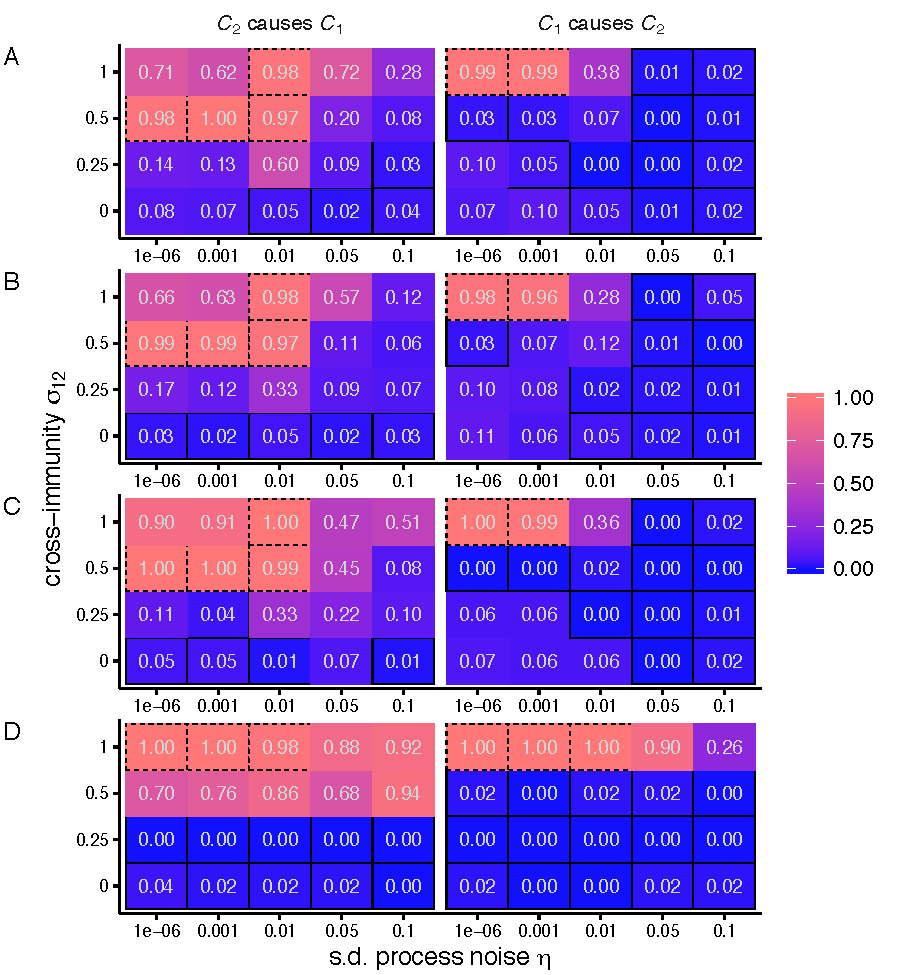
\includegraphics[width=6in]{dataflow/out/fig_detect_diffdata/fig_detect_diffdata.pdf}
  \end{center}
  \caption{\textbf{Interactions detected as a function of process noise and the strength of interaction ($C_2 \rightarrow C_1$) for different types of data}. Heat maps show the fraction of 100 replicates significant for each inferred interaction for different parameter combinations. A significant increase in cross-map correlation $\rho$ with library length $L$ indicated a causal interaction. Each analysis is based on 1000 years of data. (A) Annual incidence, (B) prevalence strobed annually, (C) first-differenced annual incidence, and (D) monthly incidence without seasonal forcing.  \label{fig:detect_diffdata}}
\end{figure}


\begin{figure}%[h]
\begin{center}
  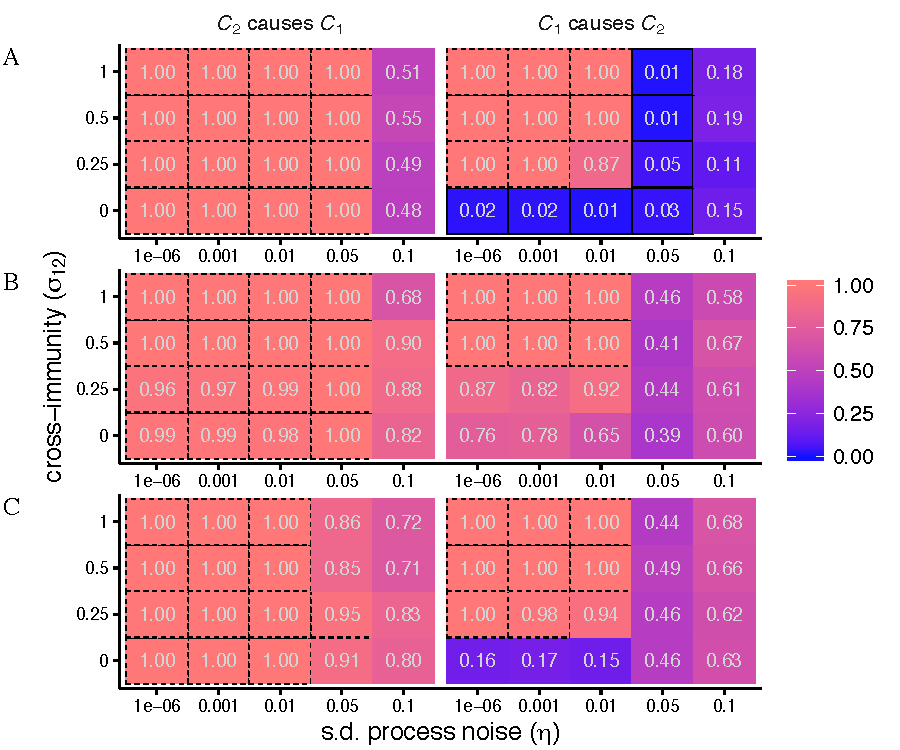
\includegraphics[width=6in]{dataflow/out/fig_detect_diffembed/fig_detect_diffembed.pdf}
  \end{center}
  \caption{\textbf{Interactions detected as a function of process noise and the strength of interaction ($C_2 \rightarrow C_1$) for different delay-embedding methods}. Heat maps show the fraction of 100 replicates significant for each inferred interaction for different parameter combinations. A significant increase in cross-map correlation $\rho$ with library length $L$ indicated a causal interaction. Each analysis is based on 100 years of monthly data. Delay-embeddings were chosen by (A) nonuniform embedding, (B) random projection, or (C) maximizing the cross-map correlation $\rho$.  \label{fig:detect_diffembed}}
\end{figure}

\begin{figure}%[h]
\begin{center}
  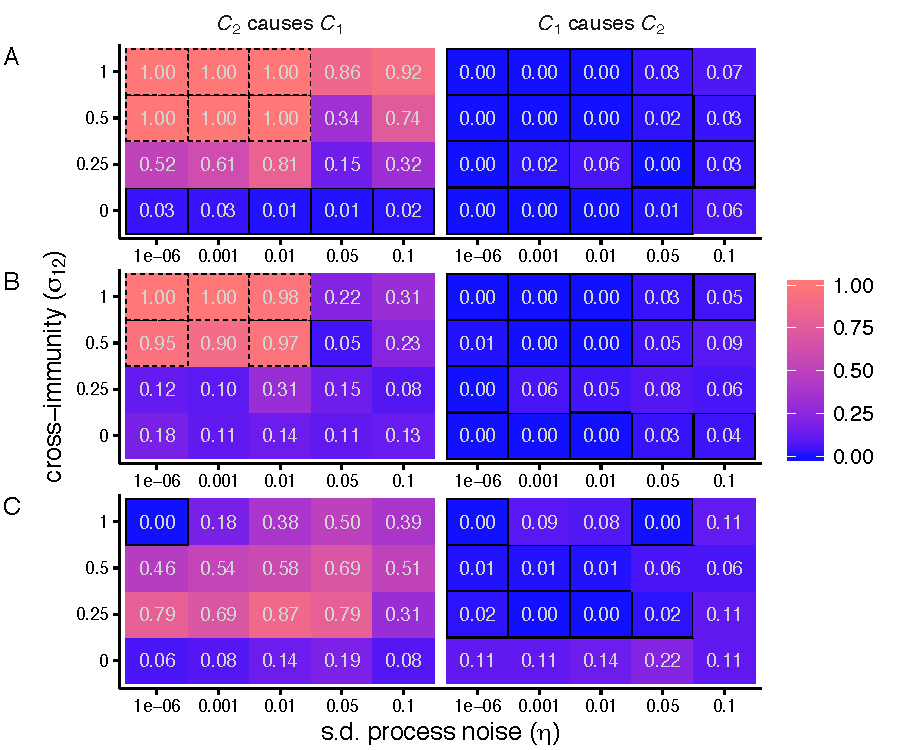
\includegraphics[width=6in]{dataflow/out/fig_detect_diffdata_lag/fig_detect_diffdata_lag.pdf}
  \end{center}
  \caption{\textbf{Interactions detected for different types of data}. Heat maps show the fraction of 100 replicates significant for each inferred interaction for different parameter combinations. A maximum cross-map correlation $\rho$ at a negative lag was required for inferring causal interaction. (A) 1000 years of annual incidence, requiring that the maximum $\rho$ be positive. (B) 100 years of monthly incidence, requiring that the maximum $\rho$ be increasing. (C) 100 years of monthly incidence with identical strains ($\beta_1=\beta_2=0.3$), requiring that maximum $\rho$ be positive.  \label{fig:detect_diffdata_lag}}
\end{figure}

\begin{figure}%[h]
\begin{center}
  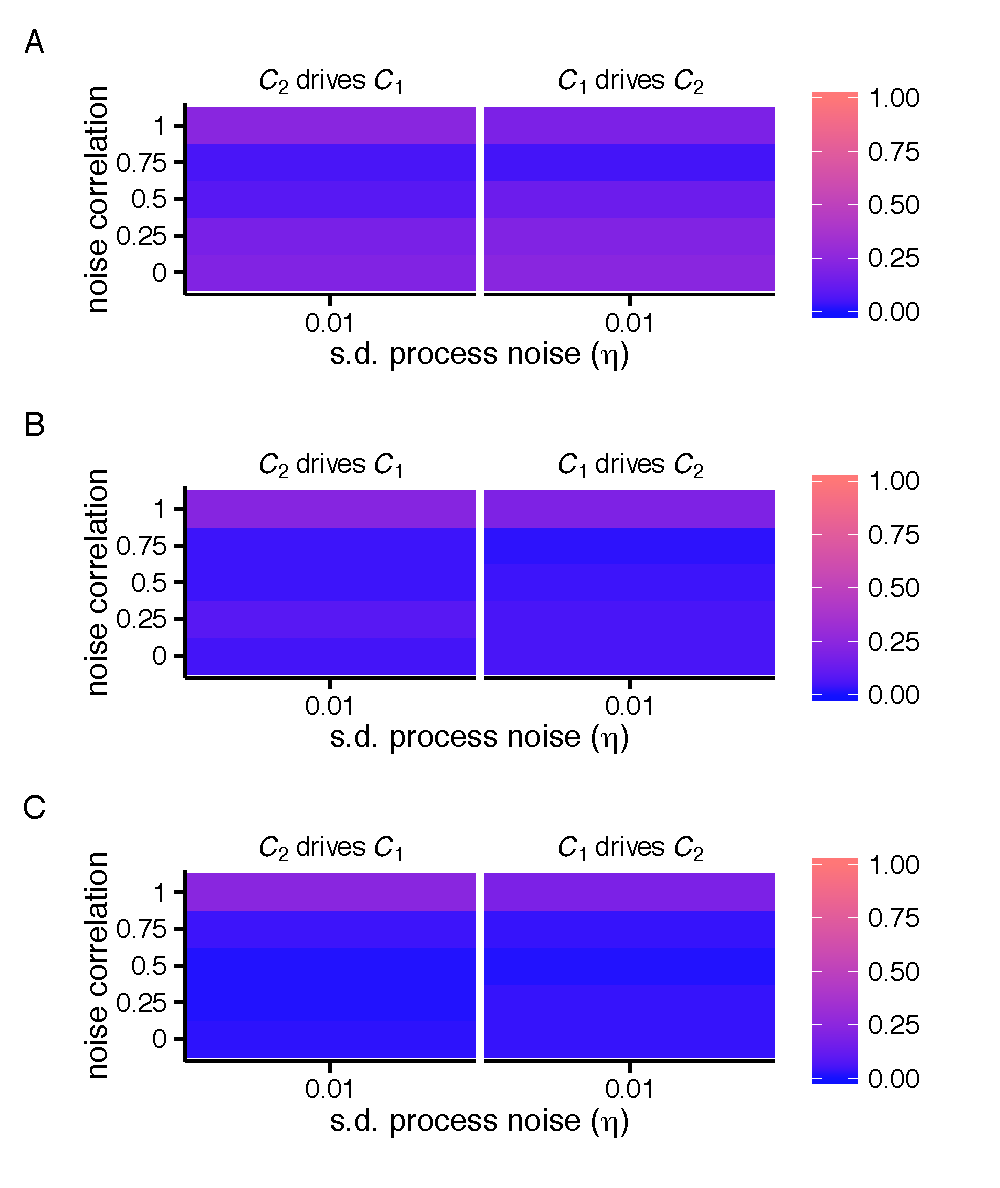
\includegraphics[width=4in]{dataflow/out/fig_detect_corrproc_identical/fig_detect_corrproc_identical.pdf}
  \end{center}
  \caption{\textbf{Interactions detected between identical strains with correlated process noise}. Heat maps show the fraction of 100 replicates significant for each inferred interaction. A maximum cross-map correlation $\rho$ at a negative lag was required for inferring causal interaction. 100 years of monthly (A) and 1000 years of annual (B) incidence, requiring that the maximum $\rho$ be positive. (C) 100 years of monthly incidence, requiring that maximum $\rho$ be increasing.  \label{fig:detect_corrproc_identical}}
\end{figure}

\begin{figure}%[h]
\begin{center}
  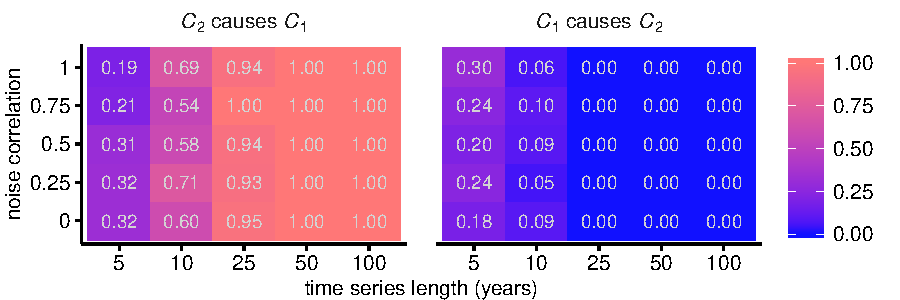
\includegraphics[width=6in]{dataflow/out/fig_detect_corrproc_distinct/fig_detect_corrproc_distinct.pdf}
  \end{center}
  \caption{\textbf{Interactions detected between distinct strains with correlated process noise}. Heat maps show the fraction of 100 replicates significant for each inferred interaction. A maximum cross-map correlation $\rho$ at a negative lag and $\rho>0$ were required for inferring causal interaction. Results are shown for 5, 10, 25, 50, and 100 years of monthly incidence.  \label{fig:detect_corrproc_distinct}}
\end{figure}

\begin{figure}
\begin{center}
  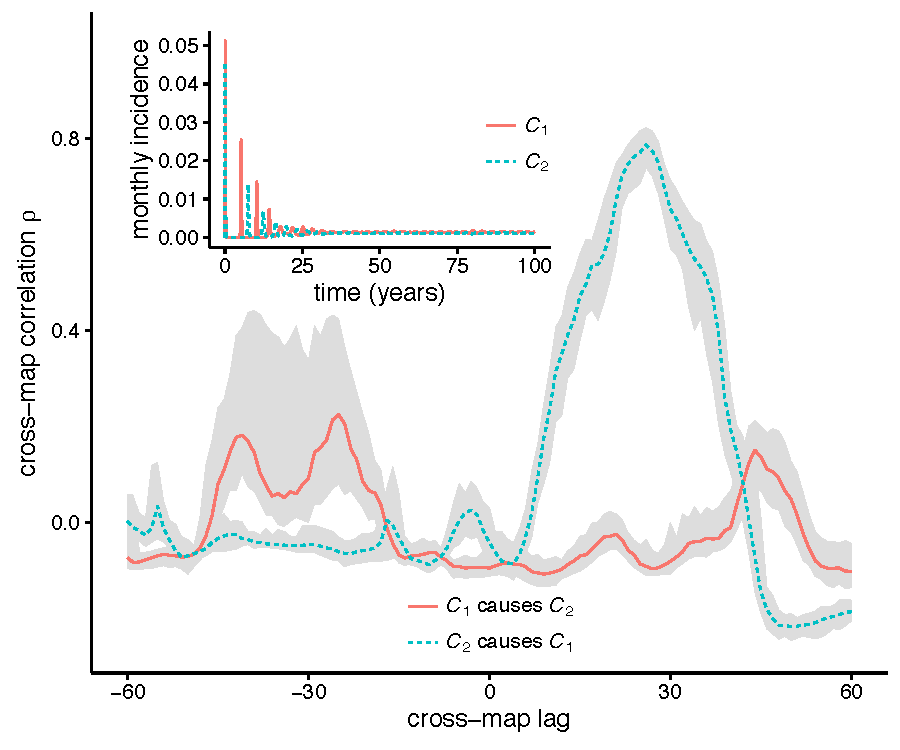
\includegraphics[width=6in]{dataflow/out/fig_transient/fig_transient.pdf}
  \end{center}
  \caption{\textbf{Incorrect inference with far-from-attractor dynamics.} Cross-map correlations at different lags for a sample 100-year time series with monthly sampling (inset). Lines represent bootstrap medians; gray ribbons represent the middle 95\% of the bootstrap distribution. Although $C_2$ drives $C_1$ ($\sigma_{12}= 0.5, \sigma_{21}=0$), the maximum cross-correlation $\rho$ for $C_1$ cross-mapped to $C_2$ occurs at a positive lag, and the reverse at a negative lag, leading to the conclusion that $C_1$ drives $C_2$, and $C_2$ does not drive $C_1$. Sample dynamics include process noise ($\eta=0.01$) but no seasonal forcing ($\epsilon=0$). \label{fig:transient}} 
\end{figure}

\begin{figure}%[h]
\begin{center}
  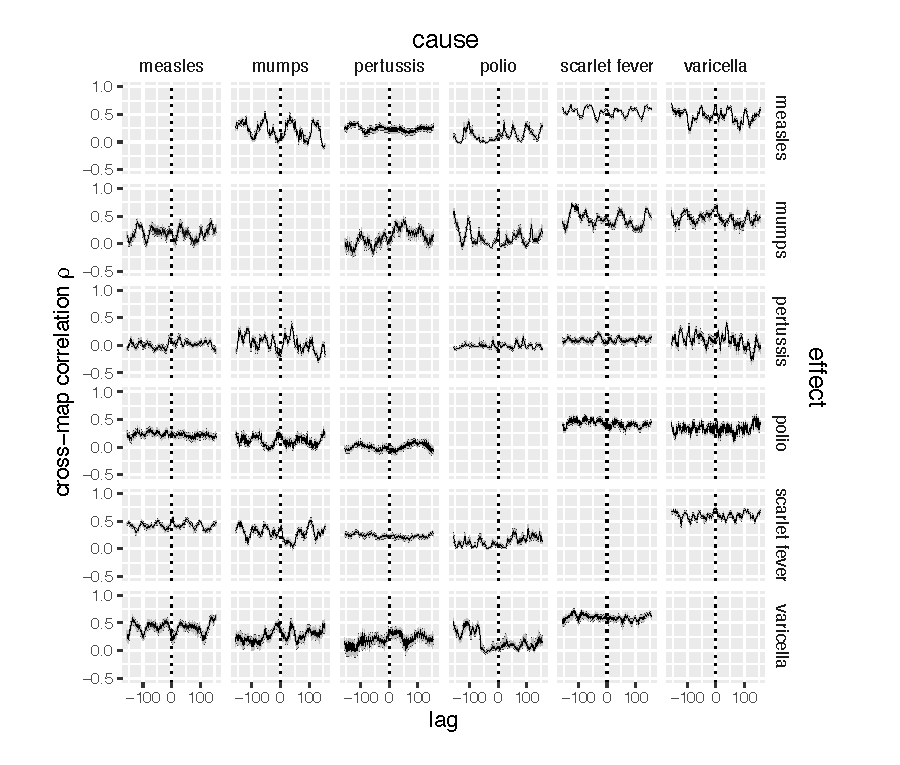
\includegraphics[width=6in]{dataflow/out/fig_cities_corrbylag/nyc_self_uniform.pdf}
  \end{center}
  \caption{\textbf{Cross-map lags for New York with default (univariate) embedding}.  \label{fig:cities_corrbylag_nyc_self_uniform}}
\end{figure}

\begin{figure}%[h]
\begin{center}
  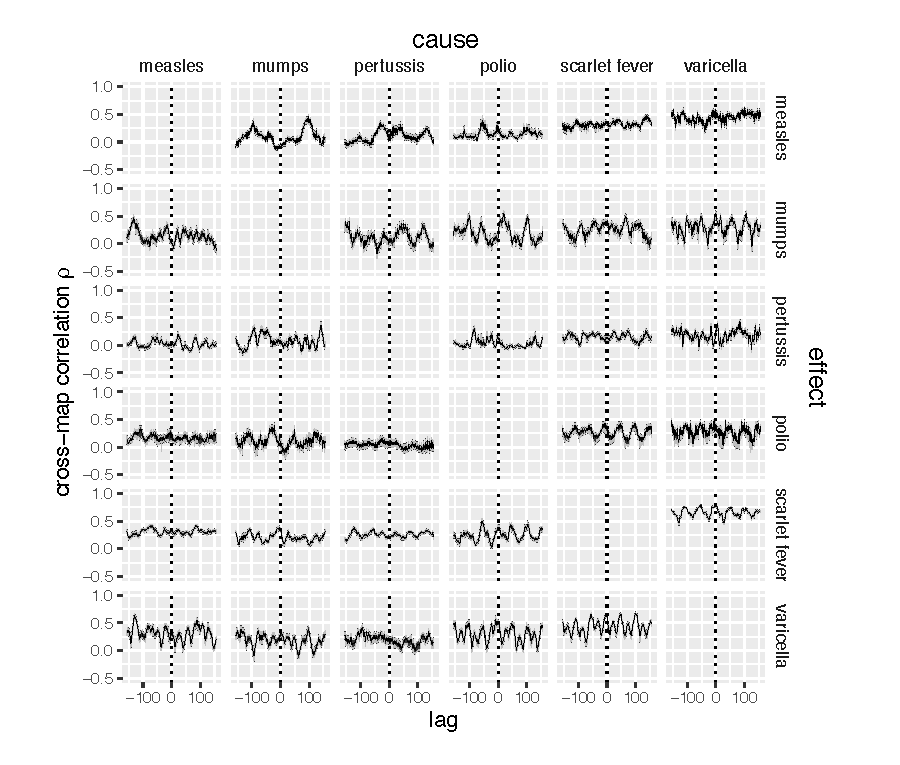
\includegraphics[width=6in]{dataflow/out/fig_cities_corrbylag/chi_self_uniform.pdf}
  \end{center}
  \caption{\textbf{Cross-map lags for Chicago with default (univariate) embedding}.  \label{fig:cities_corrbylag_chi_self_uniform}}
\end{figure}

\begin{figure}%[h]
\begin{center}
  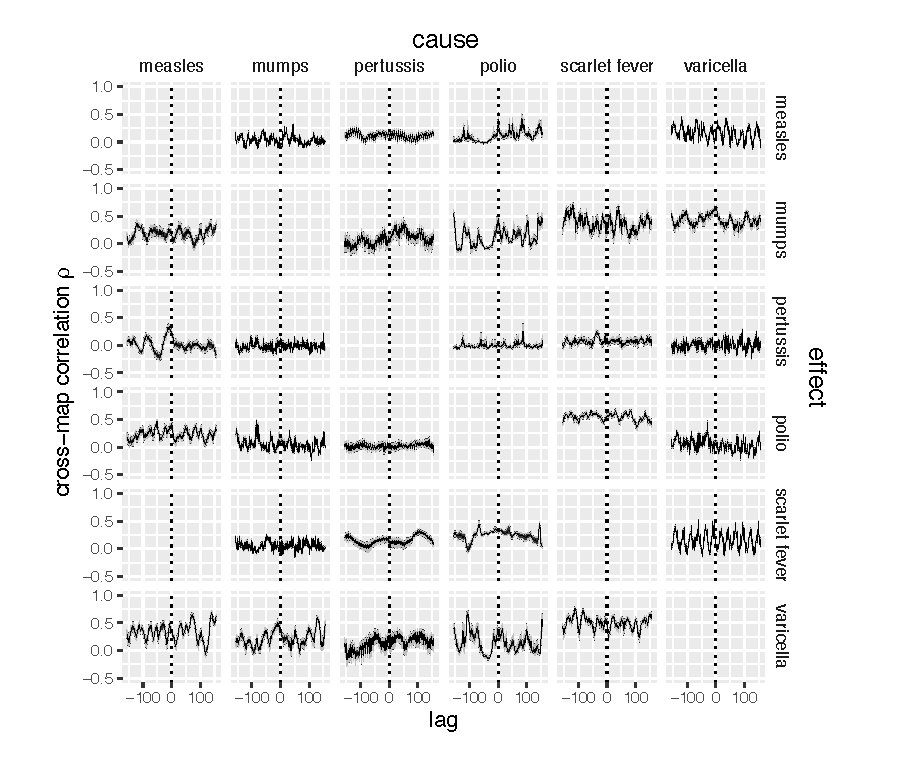
\includegraphics[width=6in]{dataflow/out/fig_cities_corrbylag/nyc_cross_projection.pdf}
  \end{center}
  \caption{\textbf{Cross-map lags for New York with embedding based on random projection}.  \label{fig:cities_corrbylag_nyc_cross_projection}}
\end{figure}

\begin{figure}%[h]
\begin{center}
  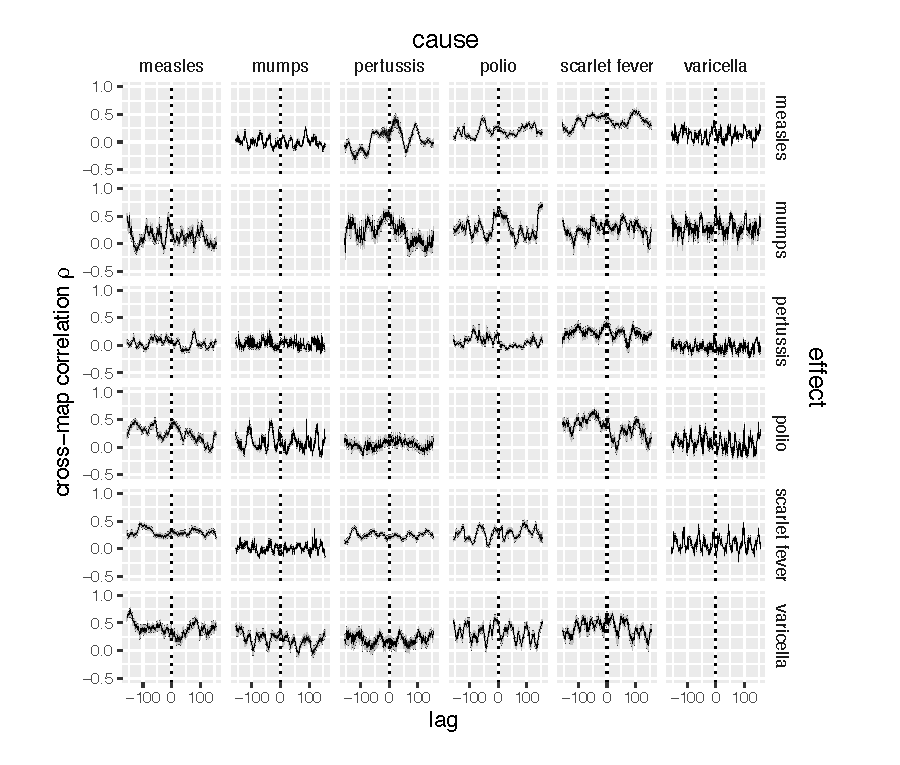
\includegraphics[width=6in]{dataflow/out/fig_cities_corrbylag/chi_cross_projection.pdf}
  \end{center}
  \caption{\textbf{Cross-map lags for Chicago with embedding based on random projection}.  \label{fig:cities_corrbylag_chi_cross_projection}}
\end{figure}
